% ---------------------------------------------------------------
% Generated by Flowchart -> TikZ Studio
% Every coordinate below is derived from the editor diagram model.
% Safe to edit by hand, but regenerating will overwrite changes.
% ---------------------------------------------------------------

\documentclass[border=8pt]{standalone}
\usepackage[T1]{fontenc}
\usepackage[utf8]{inputenc}
\usepackage{amsmath}
\usepackage{xcolor}
\usepackage{tikz}
\usetikzlibrary{shadows}

% ---- Colour definitions ----
\definecolor{fc112233}{HTML}{112233}
\definecolor{fc12161C}{HTML}{12161C}
\definecolor{fc1F2933}{HTML}{1F2933}
\definecolor{fc3366CC}{HTML}{3366CC}
\definecolor{fc35C4A8}{HTML}{35C4A8}
\definecolor{fcC0FFEE}{HTML}{C0FFEE}
\definecolor{fcDBE8FF}{HTML}{DBE8FF}
\definecolor{fcEEDDAA}{HTML}{EEDDAA}
\definecolor{fcFF8800}{HTML}{FF8800}

% ---- Style definitions ----
\tikzset{
  fcnode/.style={
    draw, inner sep=0pt, outer sep=0pt, align=center,
    line join=round, line cap=butt
  },
  fcpath/.style={line join=round, line cap=butt},
  fcedge/.style={line join=round, line cap=butt},
  fclabel/.style={inner sep=1.4pt, outer sep=0pt, align=center},
}

\begin{document}
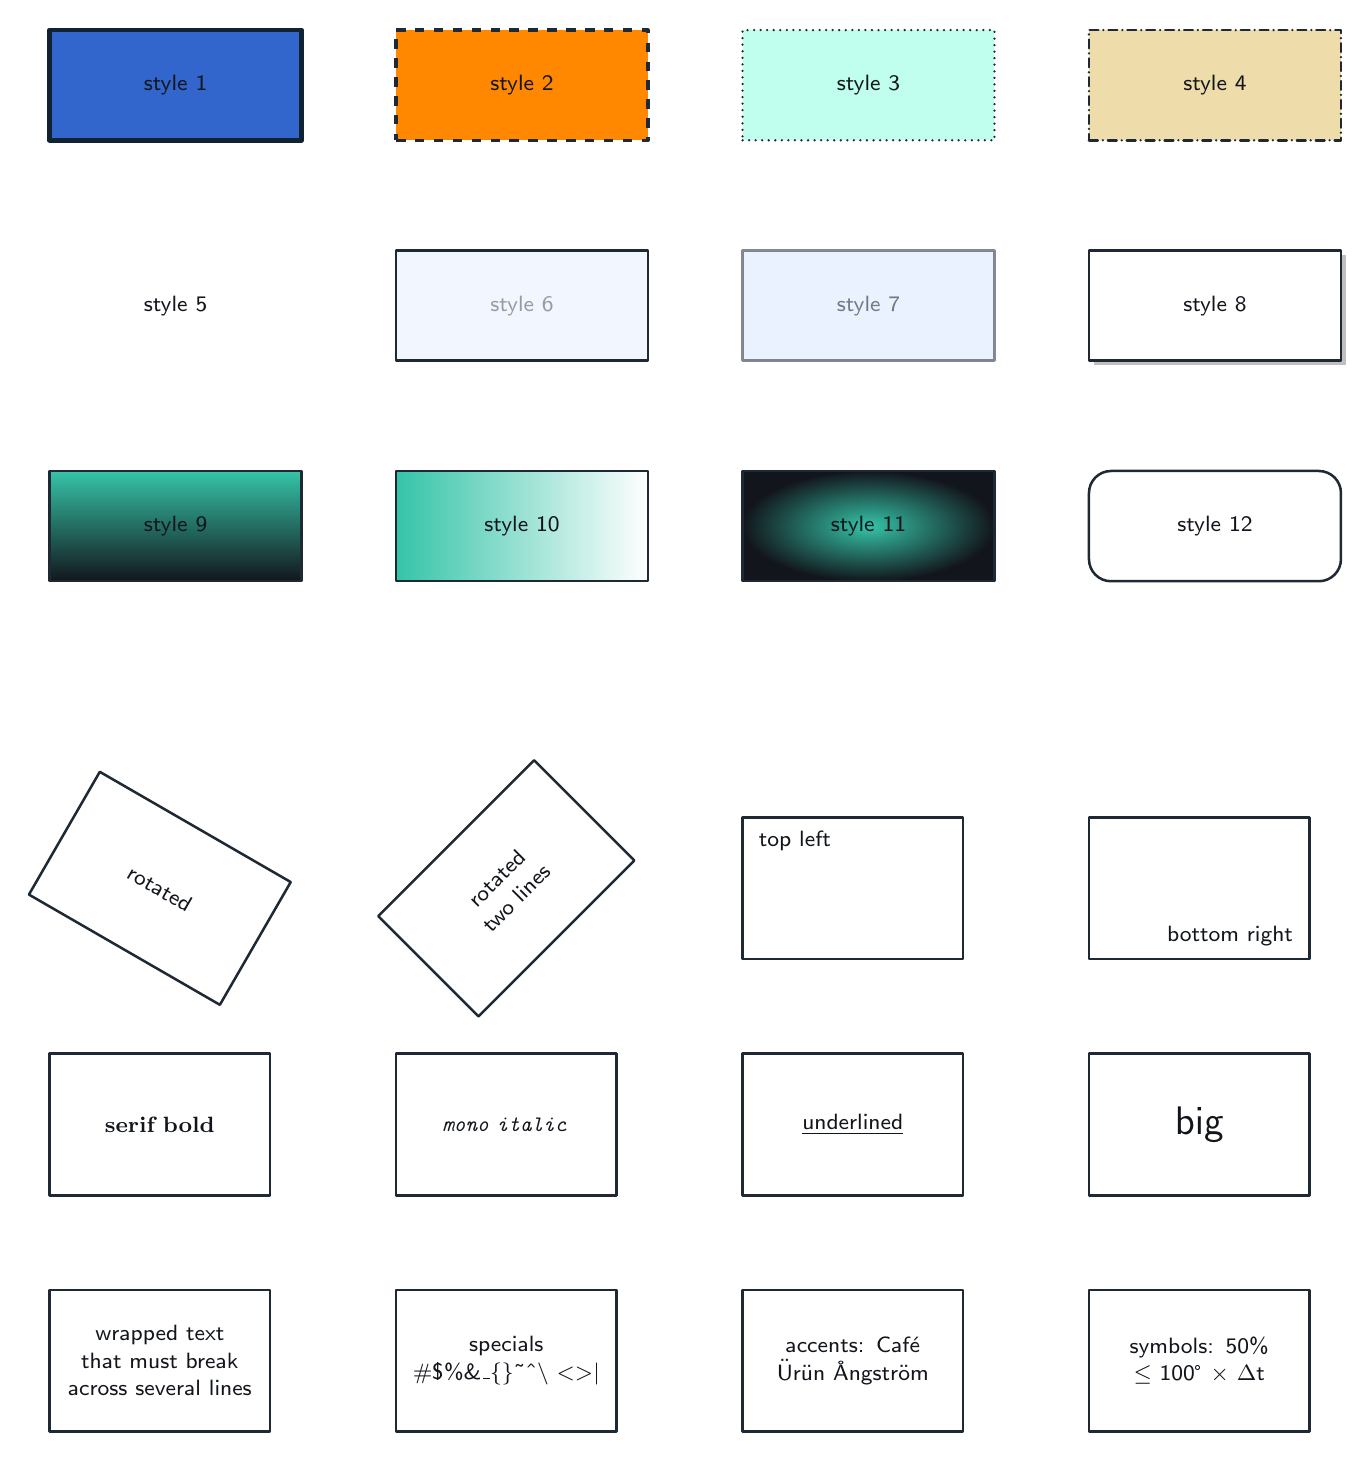
\begin{tikzpicture}[x=1cm, y=1cm]
  % ---- Nodes ----
  % n1 - Process "style 1"
  \node[fcnode, shape=rectangle, minimum width=3.2cm, minimum height=1.4cm, draw=fc112233,
        line width=1.707pt, fill=fc3366CC, font=\fontsize{7.97pt}{9.96pt}\selectfont\sffamily,
        text=fc12161C, align=center, text width=2.88cm] (n1) at (3.6,-2.7) {style 1};
  % n2 - Process "style 2"
  \node[fcnode, shape=rectangle, minimum width=3.2cm, minimum height=1.4cm, draw=fc1F2933,
        line width=1.138pt, dash pattern=on 3.414pt off 3.414pt, fill=fcFF8800,
        font=\fontsize{7.97pt}{9.96pt}\selectfont\sffamily, text=fc12161C, align=center,
        text width=2.88cm] (n2) at (8,-2.7) {style 2};
  % n3 - Process "style 3"
  \node[fcnode, shape=rectangle, minimum width=3.2cm, minimum height=1.4cm, draw=fc1F2933,
        line width=0.91pt, line cap=round, dash pattern=on 0pt off 2.367pt, fill=fcC0FFEE,
        font=\fontsize{7.97pt}{9.96pt}\selectfont\sffamily, text=fc12161C, align=center,
        text width=2.88cm] (n3) at (12.4,-2.7) {style 3};
  % n4 - Process "style 4"
  \node[fcnode, shape=rectangle, minimum width=3.2cm, minimum height=1.4cm, draw=fc1F2933,
        line width=0.91pt, line cap=round,
        dash pattern=on 3.187pt off 1.821pt on 0pt off 1.821pt, fill=fcEEDDAA,
        font=\fontsize{7.97pt}{9.96pt}\selectfont\sffamily, text=fc12161C, align=center,
        text width=2.88cm] (n4) at (16.8,-2.7) {style 4};
  % n5 - Process "style 5"
  \node[fcnode, shape=rectangle, minimum width=3.2cm, minimum height=1.4cm, draw=none,
        fill=white, font=\fontsize{7.97pt}{9.96pt}\selectfont\sffamily, text=fc12161C,
        align=center, text width=2.88cm] (n5) at (3.6,-5.5) {style 5};
  % n6 - Process "style 6"
  \node[fcnode, shape=rectangle, minimum width=3.2cm, minimum height=1.4cm, draw=fc1F2933,
        line width=0.91pt, fill=fcDBE8FF, fill opacity=0.4,
        font=\fontsize{7.97pt}{9.96pt}\selectfont\sffamily, text=fc12161C, align=center,
        text width=2.88cm] (n6) at (8,-5.5) {style 6};
  % n7 - Process "style 7"
  \node[fcnode, shape=rectangle, minimum width=3.2cm, minimum height=1.4cm, draw=fc1F2933,
        line width=0.91pt, fill=fcDBE8FF, opacity=0.55,
        font=\fontsize{7.97pt}{9.96pt}\selectfont\sffamily, text=fc12161C, align=center,
        text width=2.88cm] (n7) at (12.4,-5.5) {style 7};
  % n8 - Process "style 8"
  \node[fcnode, shape=rectangle, minimum width=3.2cm, minimum height=1.4cm, draw=fc1F2933,
        line width=0.91pt, fill=white,
        drop shadow={shadow xshift=1.707pt, shadow yshift=-1.707pt, opacity=0.25, fill=black},
        font=\fontsize{7.97pt}{9.96pt}\selectfont\sffamily, text=fc12161C, align=center,
        text width=2.88cm] (n8) at (16.8,-5.5) {style 8};
  % n9 - Process "style 9"
  \node[fcnode, shape=rectangle, minimum width=3.2cm, minimum height=1.4cm, draw=fc1F2933,
        line width=0.91pt, top color=fc35C4A8, bottom color=fc12161C,
        font=\fontsize{7.97pt}{9.96pt}\selectfont\sffamily, text=fc12161C, align=center,
        text width=2.88cm] (n9) at (3.6,-8.3) {style 9};
  % n10 - Process "style 10"
  \node[fcnode, shape=rectangle, minimum width=3.2cm, minimum height=1.4cm, draw=fc1F2933,
        line width=0.91pt, left color=fc35C4A8, right color=white,
        font=\fontsize{7.97pt}{9.96pt}\selectfont\sffamily, text=fc12161C, align=center,
        text width=2.88cm] (n10) at (8,-8.3) {style 10};
  % n11 - Process "style 11"
  \node[fcnode, shape=rectangle, minimum width=3.2cm, minimum height=1.4cm, draw=fc1F2933,
        line width=0.91pt, inner color=fc35C4A8, outer color=fc12161C,
        font=\fontsize{7.97pt}{9.96pt}\selectfont\sffamily, text=fc12161C, align=center,
        text width=2.88cm] (n11) at (12.4,-8.3) {style 11};
  % n12 - Process "style 12"
  \node[fcnode, shape=rectangle, minimum width=3.2cm, minimum height=1.4cm,
        rounded corners=0.28cm, draw=fc1F2933, line width=0.91pt, fill=white,
        font=\fontsize{7.97pt}{9.96pt}\selectfont\sffamily, text=fc12161C, align=center,
        text width=2.88cm] (n12) at (16.8,-8.3) {style 12};
  % x1 - Rectangle "rotated"
  \node[fcnode, shape=rectangle, minimum width=2.8cm, minimum height=1.8cm, draw=fc1F2933,
        line width=0.91pt, fill=white, font=\fontsize{7.97pt}{9.96pt}\selectfont\sffamily,
        text=fc12161C, align=center, text width=2.48cm, rotate=-30]
        (x1) at (3.4,-12.9) {rotated};
  % x2 - Rectangle "rotated"
  \node[fcnode, shape=rectangle, minimum width=2.8cm, minimum height=1.8cm, draw=fc1F2933,
        line width=0.91pt, fill=white, font=\fontsize{7.97pt}{9.96pt}\selectfont\sffamily,
        text=fc12161C, align=center, text width=2.48cm, rotate=45]
        (x2) at (7.8,-12.9) {rotated \\ two lines};
  % x3 - Rectangle "top left"
  \node[fcnode, shape=rectangle, minimum width=2.8cm, minimum height=1.8cm, draw=fc1F2933,
        line width=0.91pt, fill=white, font=\fontsize{7.97pt}{9.96pt}\selectfont\sffamily,
        text=fc12161C, align=left, text width=2.48cm] (x3) at (12.2,-12.9) {};
  \node[fclabel, anchor=north west, font=\fontsize{7.97pt}{9.96pt}\selectfont\sffamily,
        text=fc12161C, align=left, text width=2.48cm] at (10.96,-12.12) {top left};
  % x4 - Rectangle "bottom right"
  \node[fcnode, shape=rectangle, minimum width=2.8cm, minimum height=1.8cm, draw=fc1F2933,
        line width=0.91pt, fill=white, font=\fontsize{7.97pt}{9.96pt}\selectfont\sffamily,
        text=fc12161C, align=right, text width=2.48cm] (x4) at (16.6,-12.9) {};
  \node[fclabel, anchor=south east, font=\fontsize{7.97pt}{9.96pt}\selectfont\sffamily,
        text=fc12161C, align=right, text width=2.48cm] at (17.84,-13.68) {bottom right};
  % x5 - Rectangle "serif bold"
  \node[fcnode, shape=rectangle, minimum width=2.8cm, minimum height=1.8cm, draw=fc1F2933,
        line width=0.91pt, fill=white, font=\fontsize{7.97pt}{9.96pt}\selectfont\rmfamily,
        text=fc12161C, align=center, text width=2.48cm]
        (x5) at (3.4,-15.9) {\textbf{serif bold}};
  % x6 - Rectangle "mono italic"
  \node[fcnode, shape=rectangle, minimum width=2.8cm, minimum height=1.8cm, draw=fc1F2933,
        line width=0.91pt, fill=white, font=\fontsize{7.97pt}{9.96pt}\selectfont\ttfamily,
        text=fc12161C, align=center, text width=2.48cm]
        (x6) at (7.8,-15.9) {\textit{mono italic}};
  % x7 - Rectangle "underlined"
  \node[fcnode, shape=rectangle, minimum width=2.8cm, minimum height=1.8cm, draw=fc1F2933,
        line width=0.91pt, fill=white, font=\fontsize{7.97pt}{9.96pt}\selectfont\sffamily,
        text=fc12161C, align=center, text width=2.48cm]
        (x7) at (12.2,-15.9) {\underline{underlined}};
  % x8 - Rectangle "big"
  \node[fcnode, shape=rectangle, minimum width=2.8cm, minimum height=1.8cm, draw=fc1F2933,
        line width=0.91pt, fill=white, font=\fontsize{13.66pt}{17.07pt}\selectfont\sffamily,
        text=fc12161C, align=center, text width=2.48cm] (x8) at (16.6,-15.9) {big};
  % x9 - Rectangle "wrapped text that must break across seve"
  \node[fcnode, shape=rectangle, minimum width=2.8cm, minimum height=1.8cm, draw=fc1F2933,
        line width=0.91pt, fill=white, font=\fontsize{7.97pt}{9.96pt}\selectfont\sffamily,
        text=fc12161C, align=center, text width=2.4cm]
        (x9) at (3.4,-18.9) {wrapped text that must break across several lines};
  % x10 - Rectangle "specials #$\%&_{}~^\ <>|"
  \node[fcnode, shape=rectangle, minimum width=2.8cm, minimum height=1.8cm, draw=fc1F2933,
        line width=0.91pt, fill=white, font=\fontsize{7.97pt}{9.96pt}\selectfont\sffamily,
        text=fc12161C, align=center, text width=2.48cm]
        (x10) at (7.8,-18.9) {specials \#\$\%\&\_\{\}\textasciitilde{}\textasciicircum{}\textbackslash{} \textless{}\textgreater{}\textbar{}};
  % x11 - Rectangle "accents: Café Ürün Ångström"
  \node[fcnode, shape=rectangle, minimum width=2.8cm, minimum height=1.8cm, draw=fc1F2933,
        line width=0.91pt, fill=white, font=\fontsize{7.97pt}{9.96pt}\selectfont\sffamily,
        text=fc12161C, align=center, text width=2.48cm]
        (x11) at (12.2,-18.9) {accents: Café Ürün Ångström};
  % x12 - Rectangle "symbols: 50\% ≤ 100° × Δt"
  \node[fcnode, shape=rectangle, minimum width=2.8cm, minimum height=1.8cm, draw=fc1F2933,
        line width=0.91pt, fill=white, font=\fontsize{7.97pt}{9.96pt}\selectfont\sffamily,
        text=fc12161C, align=center, text width=2.48cm]
        (x12) at (16.6,-18.9) {symbols: 50\% $\leq$ 100\textdegree{} $\times$ $\Delta$t};
\end{tikzpicture}
\end{document}